\section{Kremowy makaron z cukinią i serem pleśniowym}
\bigskip
\small
\begin{minipage}{0.45\textwidth}
    \noindent \textbf{Czas:} 30 minut \\
    \textbf{Poziom trudności:} łatwy
\end{minipage}
\begin{minipage}{0.45\textwidth}
    \noindent \textbf{Ilość sprzątania:} średnia\\
    \textbf{Wymagany mysi sprzęt:} duża patelnia
\end{minipage}
\normalsize
\vspace{0.5cm}

\begin{multicols}{2}

\subsection*{Składniki}
\begin{itemize}
    \item 1 cebula
    \item 3 duże ząbki czosnku
    \item 1 duża cukinia lub kilka mniejszych
    \item 2-3 porcje makaronu
    \item 300 g śmietany 18\%
    \item ok. 100 g sera z niebieską pleśnią (np. Lazur, Grand Blue)
    \item przyprawy
    \item garść sera podpuszczkowego dojrzewającego (np. grana padano lub parmezan)
    \item oliwa do smażenia
    \item sól i pieprz do smaku
\end{itemize}

\columnbreak

\begin{figure}[H]
    \centering
    \fbox{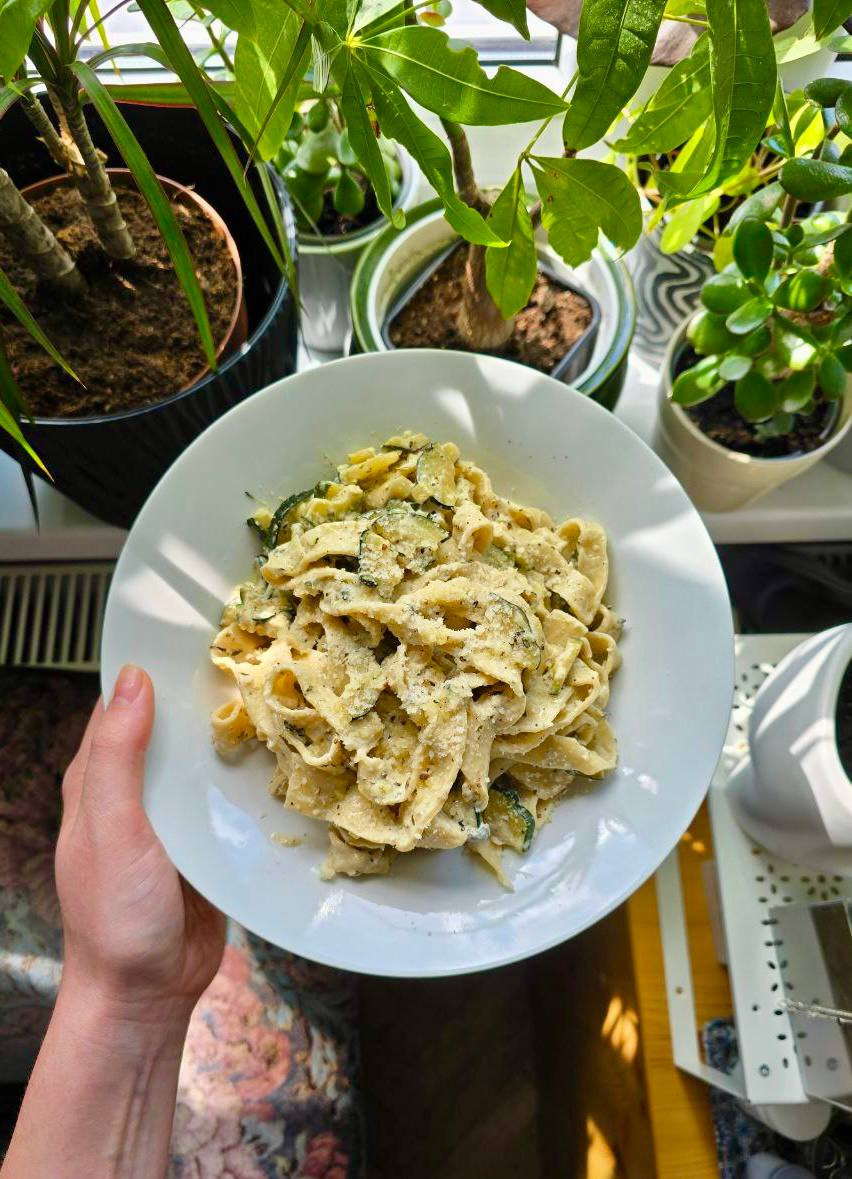
\includegraphics[width=0.4\textwidth]{images/makaron-z-cukinia.jpg}}
\end{figure}
\end{multicols}

\vspace{0.5cm}

\subsection*{Instruktaż}
\begin{enumerate}
    \item Cebulę pokroić w kostkę i zeszklić na średnim ogniu na oliwie wraz z obfitą szczyptą soli. Cukinię pokroić w półplasterki i smażyć wraz z cebulą przez ok. 5-10 minut do zauważalnego wytracenia objętości. Na ostatnie 30 sekund smażenia dodać przeciśnięty przez praskę czosnek i dokładnie wymieszać.
    \item Na patelnię wlać śmietankę, posypać płaską łyżeczką kolejno: pieprzu, bazylii, majeranku, tymianku i rozmarynu. Zmniejszyć ogień do minimalnego i wszystko dokładnie wymieszać. Dusić przez ok. 10 minut do przegryzienia sie smaków.
    \item Makaron ugotować zgodnie z instrukcją na opakowaniu. Przy odcedzaniu zachować szklankę wody z gotowania.
    \item Na koniec w sosie rozpuścić ser pleśniowy i dokładnie wymieszać. Sprawdzić smak pod kątem soli oraz pieprzu. Jeżeli konsystencja sosu jest zbyt gęsta, rozrzedzić go wodą z makaronu do uzyskania odpowiedniej gęstości.
    \item Ugotowany makaron przełożyć na patelnię i wymieszać z sosem. Gotowe danie posypać serem dojrzewającym.
\end{enumerate}

\vspace{0.5cm}

\small
\subsection*{Propozycja podania}
Z listkami świeżej bazylii lub oregano, z chluśnięciem oliwy.

\vspace{0.3cm}

\subsection*{Dodatkowe uwagi}
Jeśli pożądana jest kremowa konsystencja, sos można jak najbardziej zblendować.
